In this case, the initial voltage and SOC of the supercapacitor is set to 535V and 97.02\% respectively. The initial SOC of the battery is set at 94\%. 

In this case, the same steps of the case 1 and case 2 are performed. As seen in Fig. \ref{ch5_f117}, the simulation results up to $t$ = 2s are the same as case 1. In this case the energy storages have high SOC, so the EMS provides negative $P_{stor-ref}$ between $t$ = 1s and $t$ = 2s to meet the extra system demand from the pulsed load. But unlike case 1 and case 2 the ESM does not provide a positive $P_{stor-ref}$ for charging at $t$ = 2.5s when 4MW load is rejected and the system has excess generation to charge the energy storages. This is because the energy storages have a high SOC (nearly 97.02\% and 94\%). Similar to case 2 the EMS takes the high SOC of the energy storages into account and a zero $P_{stor-ref}$ to avoid overcharging. From the Figure \ref{ch5_f117}, it is clear that the Off-line and CHIL results are same.
  
%gfhgfhfgjhg
%fghgfhg
\begin{figure}[ht!]
\begin{subfigure}{1\columnwidth}
\begin{center}
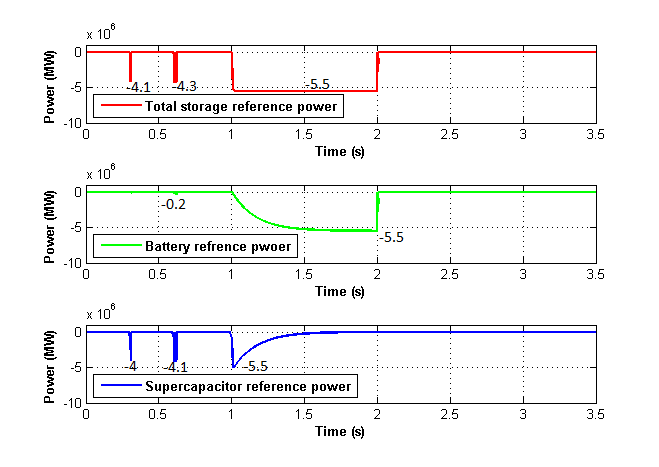
\includegraphics[height=3in, width=3.5in]{f117b}
\end{center}
\caption{Off-line simulation results.}
\label{ch5_f117b}
\end{subfigure}
\begin{subfigure}{1\columnwidth}
\begin{center}
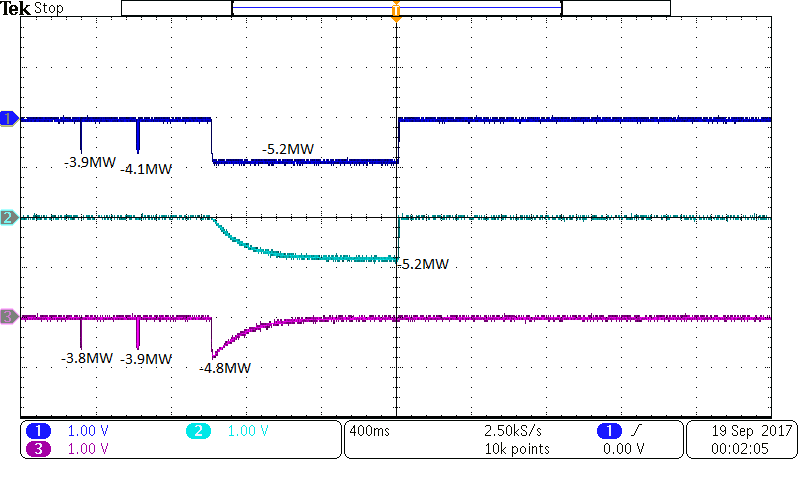
\includegraphics[height=2in, width=3.5in]{f117}
\end{center}
\caption{CHIL results-oscilloscope plots: Ch1: total storage reference power, Ch2: battery reference power, Ch3: supercapacitor reference  power (Ch1, Ch2, Ch3 = 5MW/div).}
\label{ch5_f117a}
\end{subfigure}
\caption{Reference power produced by FL controller and LPF based ESM system (case 3).}
\label{ch5_f117}
\end{figure}



